\section*{Exercice 2~: Spécification d'un protocole de communication}
\subsection*{Question 1}
\begin{center}
\begin{tikzpicture}[node distance=2cm,>=stealth',bend angle=45,auto]

  \tikzstyle{place}=[circle,thick,draw=blue!75,fill=blue!20,minimum size=6mm]
  \tikzstyle{red place}=[place,draw=red!75,fill=red!20]
  \tikzstyle{transition}=[rectangle,thick,draw=black!75,
  			  fill=black!20,minimum size=4mm]

  \tikzstyle{every label}=[red]

  \begin{scope}
    \node [place, tokens=1] (rac)      [label=above:$u-raccroche$] {};
    \node [place] (dem)      [below of=rac, label=above:$u-demLigne$]{};
    \node [transition] (acc) [below right of=dem,label=right:$acceptation$] {};
    \node [place] (conf)      [above right of=acc, label=above:$c-ConfRac$] {};
    \node [place, tokens=1] (rep)   [above of=conf,label=above:$c-repos$] {};
    \node [place] (com)  [below of=acc, label=right:$enComm$]{};
    \node [transition] (udec) [left of=rac,label=left:$uDecroche$] {};
    \node [transition] (racprem) [left of=dem,label=left:$raccPrem$] {};
    \node [transition] (confrep) [right of=rep,label=right:$confRep$]{};
    \node [transition] (racCom) [left of=com,label=left:$racCom$] {};
    \node [transition] (libe) [below of=com,label=right:$liberation$] {};
    \node [place] (faux)  [below of=libe, label=right:$enFauxAppel$] {};
    \node [transition] (racfaux) [below of=faux,label=below:$racFauxAppel$] {};

    \path[every node/.style={font=\sffamily\small}]
    (acc) 
    edge [pre] (rep)
    edge[pre](dem)
    edge [post] (com)

    (udec)
    edge [pre]                  (rac)
    edge [post]                (dem)

    (confrep)
    edge [pre]                  (conf)
    edge [post]                (rep)

    (racprem) 
    edge [pre]                  (dem)
    edge [post]                (rac)

    (racCom)
    edge [pre]                  (com)
    edge [post,bend right = 20]                (conf)
    edge [post,bend right]                (rac)

    (libe)
    edge [pre]                  (com)
    edge [post]                (faux)

    (racfaux)
    edge [pre]                  (faux)
    edge [post,bend left = 95]                (rac)
    edge [post,bend right = 85]                (conf);

  \end{scope}
  
\end{tikzpicture}
\end{center}

\subsection*{Question 2}

On veut que le réseau soit borné, cohérent et réinitialisable. Nous le
montrons par un Divide Et Impera informel. Commençons par distinguer
trois sous-réseaux~:
\begin{itemize}
\item le réseau utilisateur,
\item le réseau contrôleur,
\item le réseau synchronisé.
\end{itemize}

\begin{center}
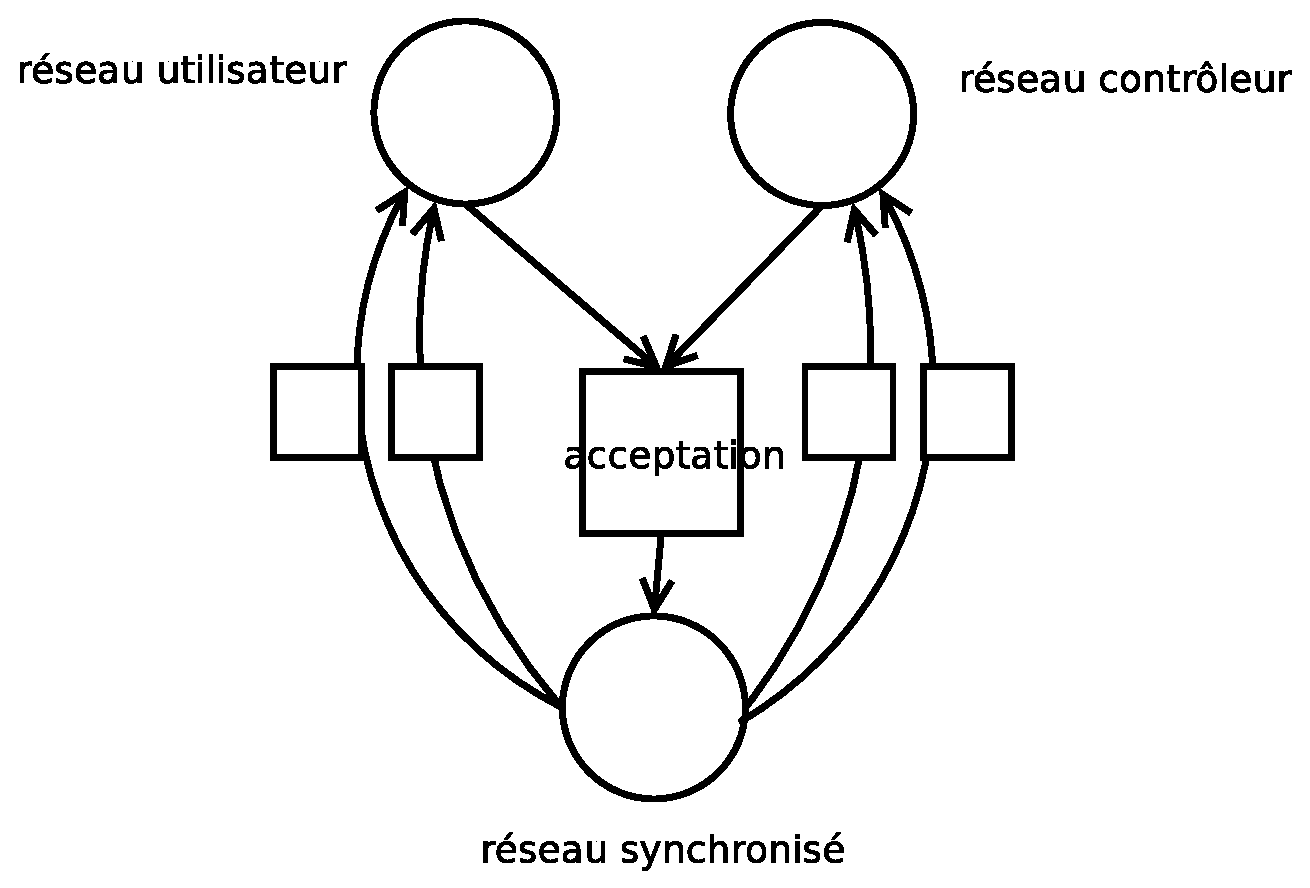
\includegraphics[width=9cm]{schemaexo2.eps}
\end{center}

Nous pouvons constater pour commencer que les jetons ne sont pas
dupliqués à l'intérieur de ces réseaux. Remarquons ensuite que le
jeton de chacun des deux réseaux parallèles ne quitte son réseaux
que de manière synchronisée avec l'autre, en passant par la transition
\textsc{acceptation}, et que cette transition produit un unique jeton
dans le réseau synchronisé.
Une fois un jeton dans le réseau synchronisé, il ne peut le quitter
qu'en produisant un jeton dans chacun des réseaux parallèles, par le
bias de \textsc{racrochage-en-communication} ou bien
\textsc{racrochage-en-faux-appel}.
Nous pouvons donc conclure que le réseau et borné et réinitialisable,
et possède soit $1$, soit $2$ jetons, suivant s'il est en mode synchronisé ou en mode parallèle~:
\begin{itemize}
\item $1$ dans chaque réseau parallèle, ou 
\item $1$ dans le réseau synchronisé.
\end{itemize} 
Nous n'avons alors qu'au plus un jeton dans chaque sous-réseau, et de
ce fait le réseau est forcément cohérent.

\subsection*{Question 3}

Notons $P_1$ la place $u-raccroche$, 

$P_2$ $\rightarrow$ $c-repos$, 

$P_3$ $\rightarrow$ $u-demLigne$, 

$P_4$ $\rightarrow$ $c-ConfRac$, 

$P_5$ $\rightarrow$ $enComm$, 

$P_6$ $\rightarrow$ $enFauxAppel$.

De même, notons $t_1$ la transition $uDecroche$, 

$t_2$ $\rightarrow$ $confRep$,

$t_3$ $\rightarrow$ $racCom$, 

$t_4$ $\rightarrow$ $acceptation$, 

$t_5$ $\rightarrow$ $racCom$, 

$t_6$ $\rightarrow$ $liberation$, 

$t_7$ $\rightarrow$ $racFauxAppel$.

Matrice $C$ d'incidence du réseau de pétri.  

 $ \begin{pmatrix}
C&t_1&t_2&t_3&t_4&t_5&t_6&t_7 \\
p_1& -1&0&1&0&1&0&1 \\
p_2&0&1&0&-1&0&0&0 \\
p_3&1&0&-1&-1&0&0&0 \\
p_4&0&-1&0&0&1&0&1 \\
p_5&0&0&0&1&-1&-1&0 \\
p_6&0&0&0&0&0&1&-1
\end{pmatrix}$


\textbf{Calcul des P-flots}


\begin{equation}
\begin{cases}
-p_1 + p_3 = 0 \\

p_2 - p_4 = 0 \\

-p_3 + p_1 = 0 \\

-p_2 - p_3 + p_5 = 0 \\

-p_5 + p_4 + p_1 = 0 \\

-p_5 + p_6 = 0 \\

 p_1 + p_4 - p_6 = 0
\end{cases}
\end{equation}

\begin{equation}
\begin{cases}
p_1 = p_3 \\

p_2 = p_4 = p_7 \\

p_5 = p_6 = p_4 + p_3
\end{cases}
\end{equation}

Donc le vecteur p-flot est~: 

($p_3,p_4,p_3,p_4,p_4 + p_3,p_4 + p_3$) $\Rightarrow$
(1,0,1,0,1,1),(0,1,0,1,1,1).


$M(p_1)+M(p_3)+M(p_5)+M(p_6)=1$


$M(p_2)+M(p_4)+M(p_5)+M(p_6)=1$

\subsection*{Question 4}

\textbf{Calcul des P semi-flots}

 $ \begin{pmatrix}
M&t_1&t_2&t_3&t_4 \\
p_1+p_3& -1&1&0&1 \\
p_2+p_4&-1&1&0&1 \\
p_5&1&-1&-1&0 \\
p_6&0&0&1&-1
\end{pmatrix}$

 $ \begin{pmatrix}
M&t_1&t_2 \\
p_1+p_3+p_5& -1&1 \\
p_2+p_4+p_5&-1&1 \\
p_6&1&-1
\end{pmatrix}$

Les P semi-flots sont donc $p_1+p_3+p_5+p_6$ et $p_2+p_4+p_5+p_6$.
